\documentclass[12pt]{article}
\usepackage{geometry}
\usepackage{graphicx}
\usepackage{amsmath}
\DeclareMathOperator{\arccsc}{arccsc}
\usepackage{hyperref}
\usepackage{sectsty}
\usepackage{cancel}
\usepackage{float}
\sectionfont{\large}
\subsectionfont{\normalsize}
\setlength{\parindent}{0cm}
\geometry{top=2.5cm,bottom=2.5cm,left=2.5cm,right=2.5cm}
\title{Golfballs in a Jar}
\author{Jim Tang}
\begin{document}

  %\begin{center} {\LARGE\textbf{Golfballs in a Jar}} \end{center}
  %\begin{center} {\large Jim Tang} \end{center}
  \maketitle

We begin with a story, found \href{http://www.lancaster.edu.mx/lancaster/Students/GRADUATION_SPEECH_2008.htm}{here}. The relevant part of it that inspires this document is as follows:
\begin{quote}
\small{Without saying a word to his students, he removed the lid of the jar and filled it with golf balls. When no more golf balls fit he closed the jar with its lid. He then asked his class, �Would you say that the jar is now full?� His students observed the jar and concluded that the jar was indeed full.

The professor then proceeded to open the jar up and started inserting marbles into the jar. The marbles started to fill the gaps between the golf balls. After sealing the jar, he asked his class once again if they thought the jar was now full. The class concluded that the jar was indeed now full.

The professor opened the jar a third time and started pouring in sand. Obviously, the sand started filling the gaps between the golf balls and the marbles. He then sealed the jar and asked his class a third time if the jar was full. His class chuckled and replied in unison, �Yes, it is now full!�

The professor opened the jar and emptied two small cups of coffee in the jar. The liquid had completely filled the gap between the golf balls, the marbles, and the grains of sand.}
\end{quote}
So the question is: how many golfballs could I potentialy fit into a jar? After I add those golfballs, how many pebbles could I fit? Then what is the volume left?

\numberwithin{equation}{section}
\numberwithin{figure}{section}
\section*{I. Golfballs}
\setcounter{section}{1}

\textbf{Approach.} We look at one dimension at a time, and assume a perfectly cylindrical jar as well as a perfectly spherical golfball. First, we divide the jar into circular layers running from the bottom to the top of the jar. For each of those layers, we divide into concentric rings. By finding the amount of balls that can `fit' into a concentric ring, summing the result over all rings of a layer, and then finally summing the result for a layer over the height of the jar, we find the total number of balls that can fit into the jar.

\vspace{10pt}\textbf{Notation.} $r_b$ = radius of golfball; $\rho$ = radius of cylindrical jar; $h$ = height of jar; $R_k$ = radius of \textit{k}th ring in a layer; $N$ = number of golfballs that fit in the jar; $N_\ell$ = number of golfballs that fit in a layer; $n_k$ = number of golfballs that fit into the \textit{k}th ring of a layer. We will introduce more variables as needed; these are the most prominent ones.

\vspace{10pt}\textbf{Approximations.} We go from the easiest to the most complex approximations. Note that for $r_g / \rho \rightarrow 0$, the actual result asymptotically approaches these approximations. The most obvious and simple one is
\begin{align} \label{eq:approx1}
N \approx \frac{\text{volume of jar}}{\text{volume of golfball}} = \frac{\pi \rho^2 h}{\frac{4}{3}\pi r_b^3} =  \frac{3}{4}\frac{\rho^2 h}{r_b^3}.
\end{align}
The next approximation is to do this layer by layer. For each layer,
\begin{align} \label{eq:approx2a}
N_\ell \approx \frac{\text{area of layer}}{\text{area of golfball cross-section}} = \frac{\pi \rho^2}{\pi r_b^2} = \left(\frac{\rho}{r_b}\right)^2.
\end{align}
The number of layers is equal to the height of the jar divided by the height of a golfball, or $h/2r_b$, a result we'll use later as well. \eqref{eq:approx2a} is valid for one layer, so we multiply that by the number of layers $h/2r_b$:
\begin{align} \label{eq:approx2}
N = \frac{h}{2r_b} N_\ell \approx \frac{1}{2}\frac{\rho^2 h}{r_b^3}.
\end{align}
A third method is to use a different volume for a golfball. Since golfballs have finite radius and cannot be packed against each other perfectly, \eqref{eq:approx1} may not be the most valid. So we replace the golfball volume with an \textit{effective} golfball volume $>$ actual volume. For this effective volume, we use a cube with sides equal to the diameter $2r_b$. From this we get that
\begin{align} \label{eq:approx3}
N \approx \frac{\text{volume of jar}}{\text{\textit{effective} volume of golfball}} = \frac{\pi \rho^2 h}{(2r_b)^3} =  \frac{\pi}{8}\frac{\rho^2 h}{r_b^3}.
\end{align}
We can go on and on by using different effective volumes, but these will be the three approximations we use for now. Note that each successive approximation reduces the prefactor to the dimensionless ratio $\rho^2 h / r_b^3$; this ratio we will denote $N_o$. 

\vspace{10pt}\textbf{The idea of resonance.} In physics, `resonance' in the spatial context occurs when a periodic disturbance of wavelength $\lambda$ exactly `fits' into a well, let's say, of length $L$. When this occurs, oscillations of high amplitude are able to form. Such phenomenon are important in many aspects of science, such as quantum mechanics, acoustics, optics, just to name a few. Resonance occurs when $L / \lambda$ = 1, 2, 3, $\ldots$ i.e. an integer.

\vspace{10pt} Why am I explaining this? Because we'll employ a similar idea in our analysis. We'll say that golfballs are \textit{resonant} with the \textit{k}th ring when an integer number of golfballs can `fit' into that ring with no extra empty space. And then we'll say that golfballs are \textit{resonant} with the container if there are an integer number of rings with even radial spacing within a layer. It can be shown that this condition holds when $\rho / r_b =$ integer.

\vspace{10pt} This is important because a resonant condition \textit{extremizes} the amount of balls that can fit, either into a ring, a layer, or within the jar itself. If the resonance condition is not met, we can only have fewer balls as the leftover space cannot accomodate an additional ball. By looking at the perfectly resonant condition, we can obtain an upper bound for the number of balls in the jar, and go from there. 

%\vspace{10pt} Our final approximation assumes complete resonance. Each ring has a circumference $2\pi R_k$, and each ball occupies an effective length of about $2r_b$. Thus,
%\begin{align*}
%n_k = \frac{\text{circumference of \textit{k}th ring}}{\text{length used up by ball}} = \frac{2 \pi R_k}{2r_b} = \frac{\pi R_k}{r_b}.
%\end{align*}
%The thickness of a ring is given by the thickness of a ball layer, the diameter of the ball itself: 2$r_b$. So the number of rings is the ratio of the radius of the container to the thickness of a ring: $\rho / 2r_b$.\footnote{This may not be an integer, and we'll revisit this issue later. For now, we will take it as an integer.} The number of balls in a layer is

\vspace{10pt}\textbf{Finding $n_k$.} Finding an exact or even a near-exact solution is rather complicated. We start by looking at an individual ring. Examine the below figure carefully, and keep in mind we are asserting the resonant condition:
\begin{figure}[H] 
  \centering 
   \includegraphics[width=0.54\textwidth]{golfball/golfball_1_cropped.jpg}
   \caption{Schematic for geometric and trigonometric calculations in this section.}
   \label{fig:calc1}
\end{figure}
%\begin{center}
%	\scalebox{0.5}{\includegraphics{C:/Users/Jim/Documents/Latex_Docs/golfball_1_cropped.jpg}}
%\end{center}
Regardless of the number of golfballs that fit along the ring, the following relation can be gleamed from the figure:
\begin{align} \label{eq:trig1}
\sin \theta = \frac{r_b}{R_k}.
\end{align}
It can also be seen that
\begin{gather*}
2n_k \theta = 2\pi, \; \; \; \text{ and} \\[0.4em]
2n_k r_b = \text{perimeter of regular polygon formed by golfballs, inscribed in \textit{k}th ring/circle}.
\end{gather*}
(As a reminder, $n_k$ is the number of golfballs that can fit into the \textit{k}th ring, and will be the number of sides of the polygon.) Taking the first condition, we get
$$
\sin \left( \frac{\pi}{n_k}\right) = \frac{r_b}{R_k},
$$
and thus, solving for $n_k$,
\begin{align} \label{eq:nkeqn1}
n_k = \frac{\pi}{\arcsin (r_b / R_k)}.
\end{align}
Our next step is to find $R_k$. Asserting the resonant condition, there are two possible cases, as shown in the next figure:
\begin{figure}[H] 
  \centering 
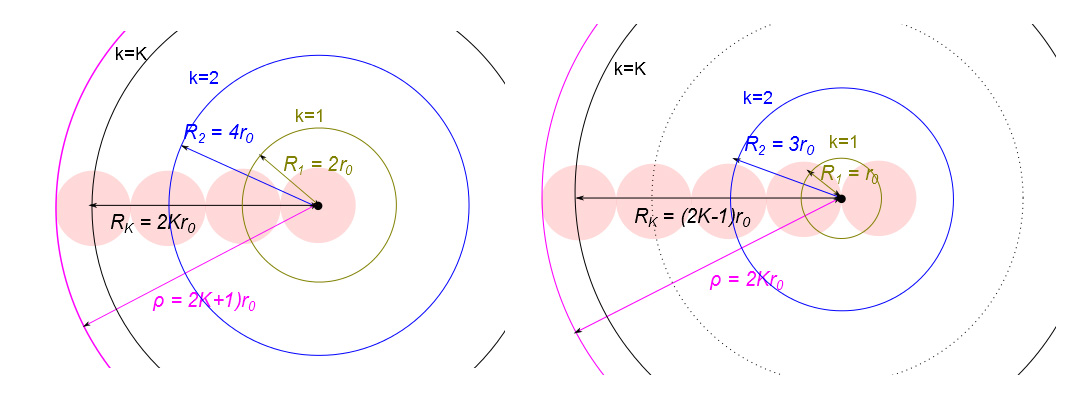
\includegraphics[width=0.99\textwidth]{golfball/golfball_2_Tot.jpg}
   \caption{Left(a): The `odd' resonant condition, where an odd number of golfball radii fit into the container. Right(b): The `even' resonant condition, where an even number of golfball radii fit. Note that $r_o = r_b$.}
   \label{fig:tworesonances}
\end{figure}
From Figure~\ref{fig:tworesonances}, we can see $R_k$ as a function of $r_b$ and $k$, for both the even and odd cases. These will be explained further below.

\vspace{10pt}\textbf{Upper bound for odd resonant case.} In this case, oddly enough, an even number of $r_b$'s fit into the \textit{k}th ring, the reasoning being the ball at $R_k = 0$ contributes one $r_b$, and the ball resting on the ring contributes another. (See Figure~\ref{fig:tworesonances}(a).) Therefore,
$$
R_k = 2kr_b \; \; \text{ and thus } \; \; \frac{r_b}{R_k} = \frac{1}{2k}.
$$
And so, denoting $n_{ko}$ as the number of balls in the \textit{k}th ring of the odd resonant case,
\begin{align} \label{eq:nkeqn1odd}
n_{ko} = \frac{\pi}{\arcsin (1/2k)}.
\end{align}
Before we sum over all the rings, we must not forget the ball in the center, which is in a peculiar situation. Recall that the arcsin only takes arguments $\leq$ 1. From \eqref{eq:nkeqn1}, this only occurs if $R_k \geq r_b$, and the ball in the center clearly has $R_k = 0$. We alleviate this situation by adding the center ball to our answer manually. There is only one ball in that center ring, so we add one.

\vspace{10pt} Finally, we see from Figure~\ref{fig:tworesonances}(a) that $\rho = (2K+1) r_b$, where $k=K$ is the maximum index that is summed. In other words, the \textit{K}th ring is the largest ring that can fit in the container. Solving for $K$, we get
$$
K = \frac{1}{2}\left(\frac{\rho}{r_b} - 1\right). 
$$
Doing the summation and adding the center ball, we get our upper-bound result
\begin{align} \label{eq:nleqn1odd}
N_{\ell o} = 1+\sum_{k=1}^{\frac{1}{2}\left(\frac{\rho}{r_b} - 1\right)} \frac{\pi}{\arcsin(1/2k)}.
\end{align}

\vspace{10pt}\textbf{Upper bound for even resonant case.} From Figure~\ref{fig:tworesonances}(b), 
$$
R_k = (2k-1)r_b \; \; \text{ and thus } \; \; \frac{r_b}{R_k} = \frac{1}{2k-1}.
$$
And so, denoting $n_{ke}$ as the number of balls in the \textit{k}th ring of the even resonant case,
\begin{align} \label{eq:nkeqn1even}
n_{ke} = \frac{\pi}{\arcsin (1/(2k-1))}.
\end{align}
We do not have to add an additional ball since the first layer rests at $R_k = r_b$. The maximum index $K$ satisfies $\rho = 2Kr_b$ (again, see Figure~\ref{fig:tworesonances}(b)). Thus
$$
K = \frac{\rho}{2r_b}.
$$
Summing,
\begin{align} \label{eq:nleqn1even}
N_{\ell e} = \sum_{k=1}^{\rho / 2r_b} \frac{\pi}{\arcsin(1/(2k-1))}.
\end{align}

\vspace{10pt}\textbf{Remarks; large $k$ limits.} Notice that we just found $N_\ell$ and went no further. It is a simple procedure to sum the result over the height of the jar, and we'll do that that when we obtain our \textit{exact} result (and later on in this section for an approximation). Meanwhile, we'll digress for a short section here to test the validity of our results, and compare them to our approximations \eqref{eq:approx1}, \eqref{eq:approx2}, \eqref{eq:approx3}. We start by Taylor expanding the arcsin:
$$
\arcsin x \approx x + \frac{x^3}{6} + \ldots
$$
For very large $k$, or very small $r_b / R_k$, the argument to the arcsin in \eqref{eq:nleqn1odd} and \eqref{eq:nleqn1even} becomes very small, and all terms of the Taylor expansion beyond 2nd order can be neglected. We are left with
$$
n_k \approx \frac{\pi}{\arcsin(1/2k)} \rightarrow 2k \pi = \text{circumference of circle with radius $k$}.
$$
This is expected. For large $k$, $R_k \gg r_b$ such that the balls in the \textit{k}th ring approach a continuum, and the spacing between rings becomes nearly negligible. Thus the amount of balls in the a ring should approach the circumference of the ring, with radius equal to $k$ because of the negligible spacing. 

\vspace{10pt} Now for the actual sum, because we are summing through so many indices, we can approximate the summation in \eqref{eq:nleqn1even} with an integral (again ignoring constant terms):
$$
N_\ell \approx \int_1^{\rho/2r_b} \frac{\pi}{\arcsin(1/2k)} \; dk \approx \int_0^{\rho/2r_b} 2 \pi k \; dk = \pi \left(\frac{\rho}{2r_b}\right)^2,
$$
where we have used our first-order result to simplify our integral, and changed our bottom limit without accruing much error, given the large $k$ limit. This procedure is justified by the following diagram:
\begin{figure}[H] \label{fig:firstorderapprox}
  \centering 
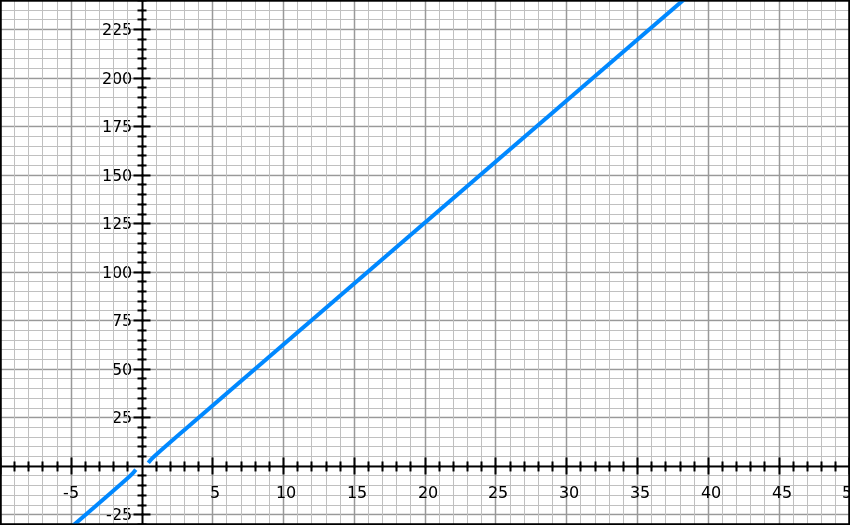
\includegraphics[width=0.43\textwidth]{golfball/graph_20120519_002016.png}
   \caption{Graph of $\pi / \arcsin(1/2x)$. Note the linear nature of the graph. \href{http://graphsketch.com/}{Link to graphing website.}}
\end{figure}
The area under the curve is very close to the triangle between two points; thus our integral is valid.
Therefore, the the number of balls in the jar, following the procedure of \eqref{eq:approx2a}, is
\begin{align} \label{eq:approx4}
N = \frac{h}{2r_b} N_\ell \approx \frac{\pi}{8} N_o.
\end{align}
(Recall $N_o$ is the ratio $\rho^2 h /r_b^3$.) Because we are using our resonant condition to formulate the result in \eqref{eq:approx4}, we can think of this result as a rough `upper bound' on valid approximations. Thus, in our approximations, it would seem only \eqref{eq:approx3} is within the valid range, and in fact, the two answers are the same. \eqref{eq:approx2} is close, but will probably be an overestimate.

\vspace{10pt}\textbf{Moving off resonance.} Resonance is hard to reach for any single ring. Using \eqref{eq:nkeqn1}, we see that for resonance to be achieved, that is for $n_k$ to indeed be an integer, $\arcsin(r_b / R_k) = \pi / I$, where $I$ is an integer greater than 1. That entails $r_b / R_k = \sin (\pi / I)$, so only select ratios of the two radii will allow resonance. These ratios are not integers, which forces us to lose both the even and odd layer resonance conditions in Figure~\ref{fig:tworesonances}. We must sacrifice ring resonance for layer resonance and vice versa; \eqref{eq:nleqn1odd} and \eqref{eq:nleqn1even} cannot possibly be exact! So we need more precise formulae valid for \textit{all} conditions.

\vspace{10pt} Off-resonance, the calculations made using Figure~\ref{fig:calc1} must be modified. Eqn \eqref{eq:trig1} is still valid, and $2\theta$ still makes up the angle formed by the two balls and the jar center (again, see Figure~\ref{fig:calc1}). However, the difference is that there are no longer an integer number of $2\theta$'s going around since there is empty spacing between two of the balls. Thus we must add a term $\alpha$ that is larger than 0 and less than 1, to account for a `fraction' of a ball in the empty space. Hence
\begin{gather*}
(n_k + \alpha)2\theta = 2\pi, \; \; \; \text{ and} \\[0.4em]
\sin \left( \frac{\pi}{n_k + \alpha} \right) = \frac{r_b}{R_k}.
\end{gather*}
So, 
\begin{align} \label{eq:nkeqn2}
n_k + \alpha = \frac{\pi}{\arcsin(r_b / R_k)}.
\end{align}
Compare to \eqref{eq:nkeqn1}. Now since $n_k$ must be an integer, and $0 < \alpha < 1$, the RHS must be less than $n_k + 1$. But we can't have a non-integer amount of balls in a ring! Therefore, we must take the closest integer \textit{less than or equal to} what we get on the RHS; this function is known as the \textit{floor}, denoted by a $\left\lfloor \; \right\rfloor$ sign around the argument. The upshot is that \eqref{eq:nkeqn2} can be rewritten as
\begin{align} \label{eq:nkeqn2b}
n_k = \left\lfloor \frac{\pi}{\arcsin(r_b / R_k)} \right\rfloor.
\end{align}
And this is the full extension of the resonant result in \eqref{eq:nkeqn1} to non-resonant cases. Notice that we are just taking the floor of the resonant result in our formulation --- this is the reason why we spent several sections on it in the first place.

\vspace{10pt}\textbf{Summing rings.} Now that we are off resonance, we have to consider how we sum the rings. We can start at the center and `stack' rings radially outward as in the resonant example, but if we are off resonance, we are going to end up with wasted space between the outer ring and the jar wall. \textit{To maximize the number of balls in a layer, we have to start by forming the outermost layer, and stacking inwards.} We'll run Figure~\ref{fig:tworesonances} backwards. Counting from the jar wall in, each \textit{k}th ring has to be centered at $\rho$ minus some odd multiple of $r_b$, starting at $\rho - r_b$. Thus
$$
\rho - (2k-1)r_b = R_k.
$$
Recall that $r_b / R_k < 1$ because arcsin only takes arguments less than unity. Therefore at max $k \equiv K$, $R_K \geq r_b$, and
$$
\rho - (2K-1)r_b \geq r_b, \; \; \text{ or } \; \;  \rho \geq 2K r_b.
$$
Hence $k \leq K \leq \rho / 2r_b$, the same result as in the even resonant case earlier. Since the indices are integers, we can also say that $K = \lfloor \rho / 2r_b \rfloor$, and this is the result we will use.

\vspace{10pt} There is one more complication, and that is the possibility of a ball resting inside $r = r_b$ in the region where \eqref{eq:nkeqn2b} is invalid (i.e. what made us consider the odd resonance). Rings are as thick as the width of the ball, i.e. the ball diameter $2r_b$. For $r_b \leq R_K < 2r_b$, there can't be another ball resting inside because the innermost ring is too thick to allow another ball inside. But for $2r_b \leq R_K < 3r_b$, another ball can fit. This must not be forgotten.

\vspace{10pt} Collecting our results, we get
\begin{gather} \label{eq:nkeqn2c}
n_k = \left\lfloor \frac{\pi}{\arcsin \left(\frac{r_b}{\rho - (2k-1)r_b} \right)} \right\rfloor = \left\lfloor \frac{\pi}{\arccsc(\rho / r_b + 1 - 2k )} \right\rfloor , \; \; \text{ and} \\[0.75em] \label{nleqn2}
N_\ell =%\sum_{k=1}^{\lfloor \rho / 2r_b \rfloor} n_k = 
\begin{cases}\displaystyle\sum\limits_{k=1}^{\lfloor \rho / 2r_b \rfloor} \left\lfloor \frac{\pi}{\arccsc(\rho / r_b + 1 - 2k )} \right\rfloor , & \text{if $r_b \leq R_{\lfloor \rho / 2r_b \rfloor} < 2r_b$} \\
	1+\displaystyle\sum\limits_{k=1}^{\lfloor \rho / 2r_b \rfloor} \left\lfloor \frac{\pi}{\arccsc(\rho / r_b + 1 - 2k )} \right\rfloor, & \text{if $2r_b \leq R_{\lfloor \rho / 2r_b \rfloor} < 3r_b$},
	\end{cases}
\end{gather}
where $R_{\lfloor \rho / 2r_b \rfloor} = R_K = \rho - (2\lfloor \rho / 2r_b \rfloor - 1)r_b$. 
%The (+1) in \eqref{eq:nkeqn2c} indicates the possibility of adding the extra ball; the cases were not presented there to conserve space. The important result is \eqref{nleqn2}.
%\begin{align}
%N_\ell = \sum_1^{\lfloor \rho / 2r_b \rfloor} n_k = 
%	\begin{cases}\sum_1^{\lfloor \rho / 2r_b \rfloor} \frac{}{} 
%	\end{cases}
%\end{align}

\vspace{10pt}\textbf{Final result.} As in previous approximations, recall we asserted that the number of layers is $h/2r_b$. However, if this ratio is not an integer, we have to take the floor, given that a layer poking out above the the container tends to spill out. Thus,
\begin{align} \label{eq:finalres}
N = \left\lfloor \frac{h}{2r_b} \right\rfloor N_\ell.
\end{align}

\vspace{10pt}\textbf{Testing our results.} Tables of values follow. The first is of $N_\ell$, the second is of $N$. 

\begin{table}[h]\footnotesize
%\caption{Table of values for $N_\ell$.}
\begin{center}
\begin{tabular}{|l|l|l|l|l|l|l|}
\hline
2$\rho$ (cm) & 2$r_b$ (cm) & $\lfloor \rho / 2r_b \rfloor$ & $n_k$ & $R_K$ & $N_\ell$ from \eqref{nleqn2} & $N_\ell$ (actual) \\ \hline
13.9 & 2.43 & 2 & $\lfloor \pi / \arccsc (6.72 - 2k) \rfloor$ & 3.31 & 23 & 24 \\ \hline
13.8 & 3.90 +/- 1.0 & 1 & $\lfloor \pi / \arccsc (4.54 - 2k) \rfloor$ & 4.95 & 8 & 8 \\ \hline
\end{tabular}
\end{center}
\end{table}
Note that the actual results differ from our thereotical results. %Explain why.

\vspace{10pt}\textbf{Finding our prefactor to $N_o$.} We see from our earlier work with large $k$ limits that $N_\ell \propto \rho^2 / r_b^2$ (roughly). Put it another way,
$$
N_\ell = \gamma \frac{\rho^2}{r_b^2},
$$
where $\gamma$ is some unknown constant, to be determined from data obtained in the previous section. Now from \eqref{eq:finalres}, and \textit{asserting only cases where $h/2r_b$ is an integer}:
$$
N = \frac{h}{2r_b} \gamma \frac{\rho^2}{r_b^2} = \frac{\gamma}{2} \frac{\rho^2 h}{r_b^3} = \frac{\gamma}{2} N_o.
$$
But $\gamma = N_\ell / (\rho / r_b)^2$. So our prefactor, using our `experimental' data, is $N_\ell / 2(\rho / r_b)^2$. Results for our $N_\ell$ data follow; the rows correspond to the rows in $N_\ell$ table in the previous section.
\begin{table}[h]\footnotesize
\begin{center}
\begin{tabular}{|l|l|l|l|}
\hline
$\rho / r_b$ & $N_\ell$ (from \eqref{nleqn2}/actual) & $\gamma$ (from \eqref{nleqn2}/actual) & prefactor (from \eqref{nleqn2}/actual) \\ \hline
5.72 & 23 / 24 & 0.70 / 0.73 & 0.35 / 0.36 \\ \hline
3.54 & 8 (same) & 0.64 & 0.32 \\ \hline 
\end{tabular}
\end{center}
\end{table}
\end{document}